\chapter{Q03}
\emph{Q3: Describe the power and energy consumption of a WSN node? How can the
energy consumption be optimized by operation? Give examples of ways to extend
the life-time of a (primary) battery based node.}

\section{Power $\slash$ energy comsumption}

\begin{figure}[h]
  \centering
  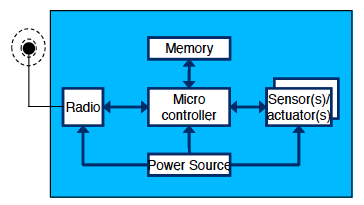
\includegraphics[scale=0.5]{img/moteAnatomy.png}
  \caption{Architecture.}
\end{figure}

\begin{description}
\item[Controller] Cheap.
\item[Radio] Expensive.
\end{description}

\subsection{States of awareness}

\begin{description}
\item Controller.
\item Radio.
\item Can react on external stimuli.
\end{description}

\section{Optimizations}
\begin{itemize}
\item Data aggregation.
\item Compute instead of transmit.
\end{itemize}
Avoid:
\begin{itemize}
\item Idle listening
\item Over-hearing.
\item Collisions (SMAC).
\end{itemize}
\begin{figure}[H]
  \centering
    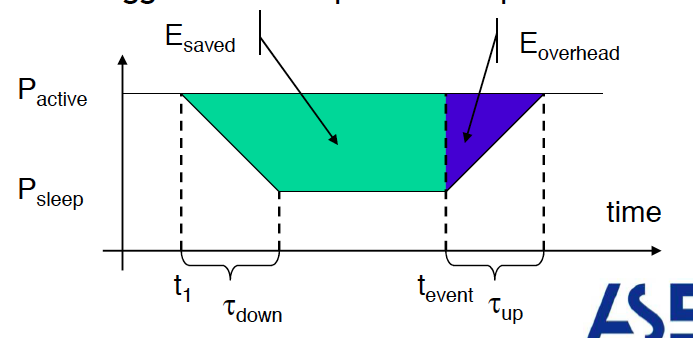
\includegraphics[scale=0.5]{img/EnergySources-DutyCycling.png}
    \caption{Duty cycling.}
\end{figure}


\section{Extending battery life}

\begin{itemize}
\item SMAC.
\item Schedule.
\item B-PHASES. Synch. Timeslots.
\item RTS.
\item CTS.
\end{itemize}

%%% Local Variables: 
%%% mode: latex
%%% TeX-master: "../master"
%%% End: 
